\documentclass[a4paper]{article}
\usepackage{pdfpages, pgffor}
\setlength{\fboxrule}{0.3mm}

\begin{document}
\newwrite\myoutput
\immediate\openout\myoutput=\jobname.options
\immediate\write\myoutput{\unexpanded{\documentclass[10pt, handout, aspectratio=169]{beamer}}} %43 for 4x3, 169 for 16x9, 1610 for 16x10
\immediate\closeout\myoutput
\foreach \n in {1,...,8}{
    \IfFileExists{week\n/week\n.tex}{
        \immediate\write18{texify.exe --pdf  --clean week\n/week\n.tex}
        \includepdf[pages=-,nup=2x2,delta=5pt 30pt,landscape=true,frame=true,column=false,noautoscale=false]{week\n.pdf}
    }
}
\end{document}

\usetheme{Frankfurt}
\usecolortheme{crane}

\usepackage{exscale,latexsym,microtype,amsmath,amssymb,amsfonts,graphicx,natbib,times,booktabs,xstring}

\newcommand{\E}{\ensuremath{{\mathbb E}}} % expected value
\newcommand{\R}{\ensuremath{{\mathbb R}}}
\newcommand{\Var}{\ensuremath{{\mathbb V}}} % variance
\newcommand{\frameit}[2]{\begin{frame}\frametitle{#1}\begin{itemize}#2\end{itemize}\end{frame}}
\def\func#1{\mathop{\rm #1}}
\def\er#1{\emph{\color{red}#1}}
\def\newblock{\hskip .11em plus .33em minus .07em}
\def\limfunc#1{\mathop{\rm #1}}%
\setbeamertemplate{blocks}[rounded][shadow=true]
\date{}

\titlegraphic{
\includegraphics[height =0.4in]{../HSLU_Logo_EN_Schwarz_rgb}}
\title{Module 9.3: Time Series Analysis with Python\\Fall Term\space\number\year}
\def\theweek{\StrRight{\jobname}{1}}
\author[Week \theweek]{\textbf{Week \theweek}:}
\AtBeginSection{
\frame{
\frametitle{Outline}
\tableofcontents[currentsection]
}}


\institute{{\Large Value at Risk}}
\begin{document}
\frame{\titlepage}
\begin{frame}%
\frametitle{Outline in Weeks}
\begin{enumerate}
\item Introduction; Descriptive Modeling
\item Returns; Autocorrelation; Stationarity
\item ARMA Models
\item Unit Roots; ARIMA Models
\item Volatility Modeling
\item Value at Risk
\item Cointegration
%\item Panel Data
\end{enumerate}
\end{frame}% 


\section[VaR]{Value at Risk (VaR)}\subsection*{}

%TCIMACRO{\TeXButton{BeginFrame}{\begin{frame}}}%
%BeginExpansion
\begin{frame}%
%EndExpansion

\frametitle{Value at Risk}

\begin{itemize}
\item Consider a portfolio with value $V_{PF,t}$ and daily returns $%
R_{PF,t+1}$.

\item Define the one-day loss on the portfolio as%
\begin{equation*}
\$Loss_{t+1}=V_{PF,t}-V_{PF,t+1}.
\end{equation*}

\item The one-day, $100\cdot p\%$, dollar \emph{\color{red}Value at Risk }$%
(\$VaR_{t+1}^{p})$ is the daily loss which will only be exceeded on the worst $100\cdot p \%$ of days. Usually, $p=0.01$.

\item Mathematically, it is the value of $\$VaR_{t+1}^{p}$ such that
%\begin{equation*}
%\mathbb{P} (\$Loss_{t+1}\leq \$VaR_{t+1}^{p})=1-p,
%\end{equation*}%
%or equivalently
\begin{equation*}
\mathbb{P} (\$Loss_{t+1}>\$VaR_{t+1}^{p})=p.
\end{equation*}
\end{itemize}

%TCIMACRO{\TeXButton{EndFrame}{\end{frame}}}%
%BeginExpansion
\end{frame}%
%EndExpansion

%TCIMACRO{\TeXButton{BeginFrame}{\begin{frame}}}%
%BeginExpansion
\begin{frame}%
%EndExpansion

\frametitle{Value at Risk}

\begin{itemize}
\item It is usually easier to express the VaR as a percentage of the portfolio value:
\begin{equation*}
VaR_{t+1}^{p}=\frac{\$VaR_{t+1}^{p}}{V_{PF,t}}.
\end{equation*}

\item Hence
\begin{equation*}
\mathbb{P} (R_{PF,t+1}<-VaR_{t+1}^{p})=p,
\end{equation*}%
as
\begin{equation*}
R_{PF,t+1}=-\frac{\$Loss_{t+1}}{V_{PF,t}}.
\end{equation*}

\item Thus $VaR_{t+1}^{p}$ is minus the $100p$th \emph{\color{red}percentile}
of the return distribution.

\item Definition can be naturally extended to $K$-day VaR, from the
distribution of the $K$-day returns $R_{PF,t+1:t+K}$.
\end{itemize}

%TCIMACRO{\TeXButton{EndFrame}{\end{frame}}}%
%BeginExpansion
\end{frame}%
%EndExpansion

%TCIMACRO{\TeXButton{BeginFrame}{\begin{frame}}}%
%BeginExpansion
\begin{frame}%
%EndExpansion

\begin{block}{Probability density function of daily returns}
\centerline{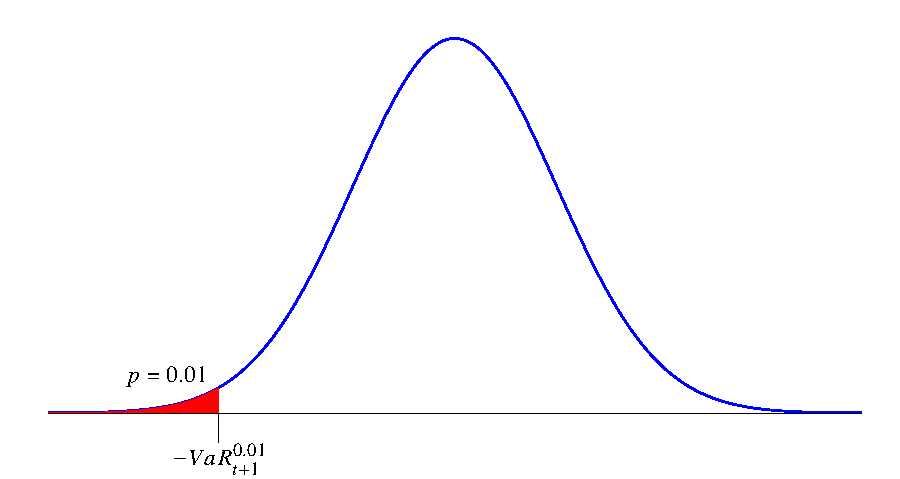
\includegraphics[height=2.3in]{density}}
\end{block}

%TCIMACRO{\TeXButton{EndFrame}{\end{frame}}}%
%BeginExpansion
\end{frame}%
%EndExpansion

%TCIMACRO{\TeXButton{BeginFrame}{\begin{frame}}}%
%BeginExpansion
\begin{frame}%
%EndExpansion

\frametitle{Value at Risk}

\begin{itemize}
\item Value at Risk was proposed as the standard measure of portfolio risk
by the Basel Committee of the Bank of International Settlements in 1996.

\item The BC imposed that financial institutions should report the Value at
Risk on their positions, such that regulators could check the adequacy of
the economic capital as a buffer against market risk.

\item Banks were allowed to use their own, internal models for the
computation of VaR, but the adequacy of these models should be
\textquotedblleft backtested\textquotedblright\ using specific criteria.

\item A candidate for a standard model is RiskMetrics (developed by
J.P.Morgan).
\item VaR is being replaced by the expected shortfall (ES) with the rollout of Basel 3. The ES is based on the VaR, however.
\end{itemize}

%TCIMACRO{\TeXButton{EndFrame}{\end{frame}}}%
%BeginExpansion
\end{frame}%
%EndExpansion
\section[Historical Simulation]{VaR Methods: Historical simulation}\subsection*{}

%TCIMACRO{\TeXButton{BeginFrame}{\begin{frame}}}%
%BeginExpansion
\begin{frame}%
%EndExpansion

\frametitle{VaR Methods: Historical simulation}

Historical simulation assumes that the distribution of tomorrow's portfolio
returns is well approximated by the empirical distribution (histogram) of
the past $m$ observations $\left\{
R_{PF,t},R_{PF,t-1},\ldots,R_{PF,t+1-m}\right\} $.

This is as if we draw, with replacement, from the last $m$ returns and use
this to simulate the next day's return distribution.

\begin{itemize}
\item The estimator of VaR is given by minus the $100p$th percentile of the
sequence of past portfolio returns, that is:

\begin{itemize}
\item sort the returns $\left\{ R_{PF,t},R_{PF,t-1},...,R_{PF,t+1-m}\right\}$
is ascending order;

\item define $R_{t+1}^{p}$ as the number such that $100p\%$ of the
observations are smaller than $R_{t+1}^{p}$;

\item the estimator for VaR is given by
\begin{equation*}
\widehat{VaR}_{t+1}^{p}=-R_{t+1}^{p}.
\end{equation*}
\end{itemize}

\end{itemize}

%TCIMACRO{\TeXButton{EndFrame}{\end{frame}}}%
%BeginExpansion
\end{frame}%
%EndExpansion

%TCIMACRO{\TeXButton{BeginFrame}{\begin{frame}}}%
%BeginExpansion
\begin{frame}%
%EndExpansion

\frametitle{VaR Methods: Historical simulation}

Problems / limitations of historical simulation:

\begin{itemize}
\item Last year(s) of data not necessarily representative for the next few
days (e.g., because of volatility clustering).

\item Similar problems as historical volatility (choice of $m$).

\item A large $m$ is required to compute the $1\%$ VaR with any degree of
precision, since we are effectively using only 1\% of the data to estimate it.

%\item By focussing on left tails, extreme positive returns are ignored.
\end{itemize}

%TCIMACRO{\TeXButton{EndFrame}{\end{frame}}}%
%BeginExpansion
\end{frame}%
%EndExpansion

\section[Normal Distribution]{VaR Methods: Normal distribution}\subsection*{}

%TCIMACRO{\TeXButton{BeginFrame}{\begin{frame}}}%
%BeginExpansion
\begin{frame}%
%EndExpansion

\frametitle{VaR Methods: Normal distribution}
\begin{itemize}
\item Another simple approach is to
assume $R_{t+1}=R_{PF,t+1}\sim N(\mu ,\sigma ^{2})$ and to estimate $\mu $
and $\sigma ^{2}$ using historical data.

%\item The VaR is then determined from%
%\begin{eqnarray*}
%\mathbb{P} \left( R_{t+1}<-VaR_{t+1}^{p}\right) &=&\mathbb{P} \left( \frac{R_{t+1}-\mu }{%
%\sigma }<\frac{-VaR_{t+1}^{p}-\mu }{\sigma }\right) \\
%&=&\mathbb{P} \left( z_{t+1}<\frac{-VaR_{t+1}^{p}-\mu }{\sigma }\right) \\
%&=&\Phi \left( \frac{-VaR_{t+1}^{p}-\mu }{\sigma }\right) =p,
%\end{eqnarray*}%
%where $\Phi (z)$ is the cumulative standard normal distribution.
\item Denoting the inverse distribution function (quantile function) of the normal as $\Phi _{p}^{-1}$, The VaR becomes
\begin{equation*}
VaR_{t+1}^{p}=-\mu -\sigma \Phi _{p}^{-1}.
\end{equation*}%
For example, $\Phi _{.01}^{-1}=-2.326$. For daily data one might take $\mu =0$.
\end{itemize}

%TCIMACRO{\TeXButton{EndFrame}{\end{frame}}}%
%BeginExpansion
\end{frame}%
%EndExpansion
%TCIMACRO{\TeXButton{BeginFrame}{\begin{frame}}}%
%BeginExpansion
\begin{frame}%
%EndExpansion

\frametitle{VaR Methods: Normal distribution}

\begin{itemize}


\item The normal model can be easily extended to a \emph{\color{red}%
conditionally} normal model. Assume $R_{t+1}\sim N(\mu_{t+1},\sigma
_{t+1}^{2}) $ where $\sigma _{t+1}^{2}$ may be estimated by:

\begin{itemize}
\item rolling windows;

\item EWMA / RiskMetrics;

\item univariate GARCH;

%\item multivariate GARCH.
\end{itemize}
\item $\mu_{t+1}$ is often just the mean return (e.g., the intercept in the mean equation for a GARCH model)
\item The VaR then becomes $VaR_{t+1}^{p}=-\mu_{t+1}-\sigma _{t+1}\Phi _{p}^{-1}$.
\end{itemize}

%TCIMACRO{\TeXButton{EndFrame}{\end{frame}}}%
%BeginExpansion
\end{frame}%
%EndExpansion


%\section{QQ plots}\subsection*{}
%
%%TCIMACRO{\TeXButton{BeginFrame}{\begin{frame}}}%
%%BeginExpansion
%\begin{frame}%
%%EndExpansion
%
%\frametitle{QQ plots}
%
%\begin{itemize}
%\item The VaR Methods described on the previous slides require that
%financial returns are either marginally or conditionally normal.
%
%\item This can be tested by performing the Jarque-Bera test.
%
%\item Another technique to compare the empirical distribution with a
%theoretical distribution is via a \emph{\color{red}QQ-plot}.
%
%\item First, the empirical distribution function of a sample $%
%\{z_{i},i=1,\ldots ,T\}$, say, $\hat{F}(z)$, is defined as the
%percentage of observations less than or equal to $z$ (for all $z\in
%\mathbb{R}$), i.e., with $z_{(i)}$ denoting the sample sorted in
%ascending fashion,
%\[
%\hat{F}(z_{(i)})=i/T.
%\]
%
%\item We can compare $\hat{F}$ to a theoretical distribution function, such
%as the standard normal $\Phi (z)$, by plotting both as functions of $z$.
%\end{itemize}
%
%%TCIMACRO{\TeXButton{EndFrame}{\end{frame}}}%
%%BeginExpansion
%\end{frame}%
%%EndExpansion
%
%%TCIMACRO{\TeXButton{BeginFrame}{\begin{frame}}}%
%%BeginExpansion
%\begin{frame}%
%%EndExpansion
%
%\begin{block}{Empirical and $N(0,1)$ distribution function of standardized returns}
%\centerline{\includegraphics[height=2.1in]{CDF.jpg}}
%\end{block}
%
%%TCIMACRO{\TeXButton{EndFrame}{\end{frame}}}%
%%BeginExpansion
%\end{frame}%
%%EndExpansion
%
%%TCIMACRO{\TeXButton{BeginFrame}{\begin{frame}}}%
%%BeginExpansion
%\begin{frame}%
%%EndExpansion
%
%\frametitle{QQ plots}
%
%\begin{itemize}
%\item A QQ plot is cross-plot (scatter diagram) of the empirical quantiles $%
%\hat{F}_{p}^{-1}$ against the standard normal quantiles $\Phi
%_{p}^{-1}$ for the observed values of $p_{i}=\hat{F}(z_{(i)})=i/T$.
%
%\item If the distributions agree, then the QQ plot should lie on the
%45-degree line.
%
%\item Fat tails correspond to a QQ plot below the 45-degree line for large
%negative values, and above the line for large positive values.
%
%\item \emph{Note}: the above comments apply to the standard definition QQ
%plots, also used in Christoffersen's book. In EViews, the axes are reversed.
%
%\item The same technique can be used to compare with other distributions
%than the standard normal.
%\end{itemize}
%
%%TCIMACRO{\TeXButton{EndFrame}{\end{frame}}}%
%%BeginExpansion
%\end{frame}%
%%EndExpansion
%
%%TCIMACRO{\TeXButton{BeginFrame}{\begin{frame}}}%
%%BeginExpansion
%\begin{frame}%
%%EndExpansion
%
%\begin{block}{QQ plots of unconditional (left) and GARCH (right) standardized returns}
%\centerline{\includegraphics[height=1.9in]{QQ.jpg}}
%\end{block}
%
%%TCIMACRO{\TeXButton{EndFrame}{\end{frame}}}%
%%BeginExpansion
%\end{frame}%
%%EndExpansion
\section[$t$ Distribution]{VaR Methods: Standardized $t$ distribution}\subsection*{}

%TCIMACRO{\TeXButton{BeginFrame}{\begin{frame}}}%
%BeginExpansion
\begin{frame}%
%EndExpansion

\frametitle{VaR Methods: Standardized $t$ distribution}

\begin{itemize}
\item The VaR methods described on the previous slides are only applicable if the
returns are normally distributed.

\item This can be tested by the Jarque-Bera test and is usually rejected.
\item Solution: use Student's $t(d)$ distribution, where d.o.f. $d>0$ need not be integer.

\item $d$ is just a shape parameter. Small values correspond to fat tails. As $d\rightarrow \infty $, we approach the $N(0,1)$ distribution.
\item For $d>2$, the variance of a $t(d)$ random variable $x$ is $d/(d-2)$;
the distribution of
\begin{equation*}
z=\frac{x}{\sqrt{\mathsf{var}(x)}}=\sqrt{\frac{d-2}{d}}x
\end{equation*}
is called \emph{\color{red}standardized }$t(d)$, denoted $\tilde{t}(d)$.

\item For $d>4$ the excess kurtosis is $6/(d-4)$. The distributions are
symmetric around $0$ (hence mean and skewness are $0$).
\end{itemize}

%TCIMACRO{\TeXButton{EndFrame}{\end{frame}}}%
%BeginExpansion
\end{frame}%
%EndExpansion

%TCIMACRO{\TeXButton{BeginFrame}{\begin{frame}}}%
%BeginExpansion
\begin{frame}%
%EndExpansion

\begin{block}{Student's $t$ densities}
\centerline{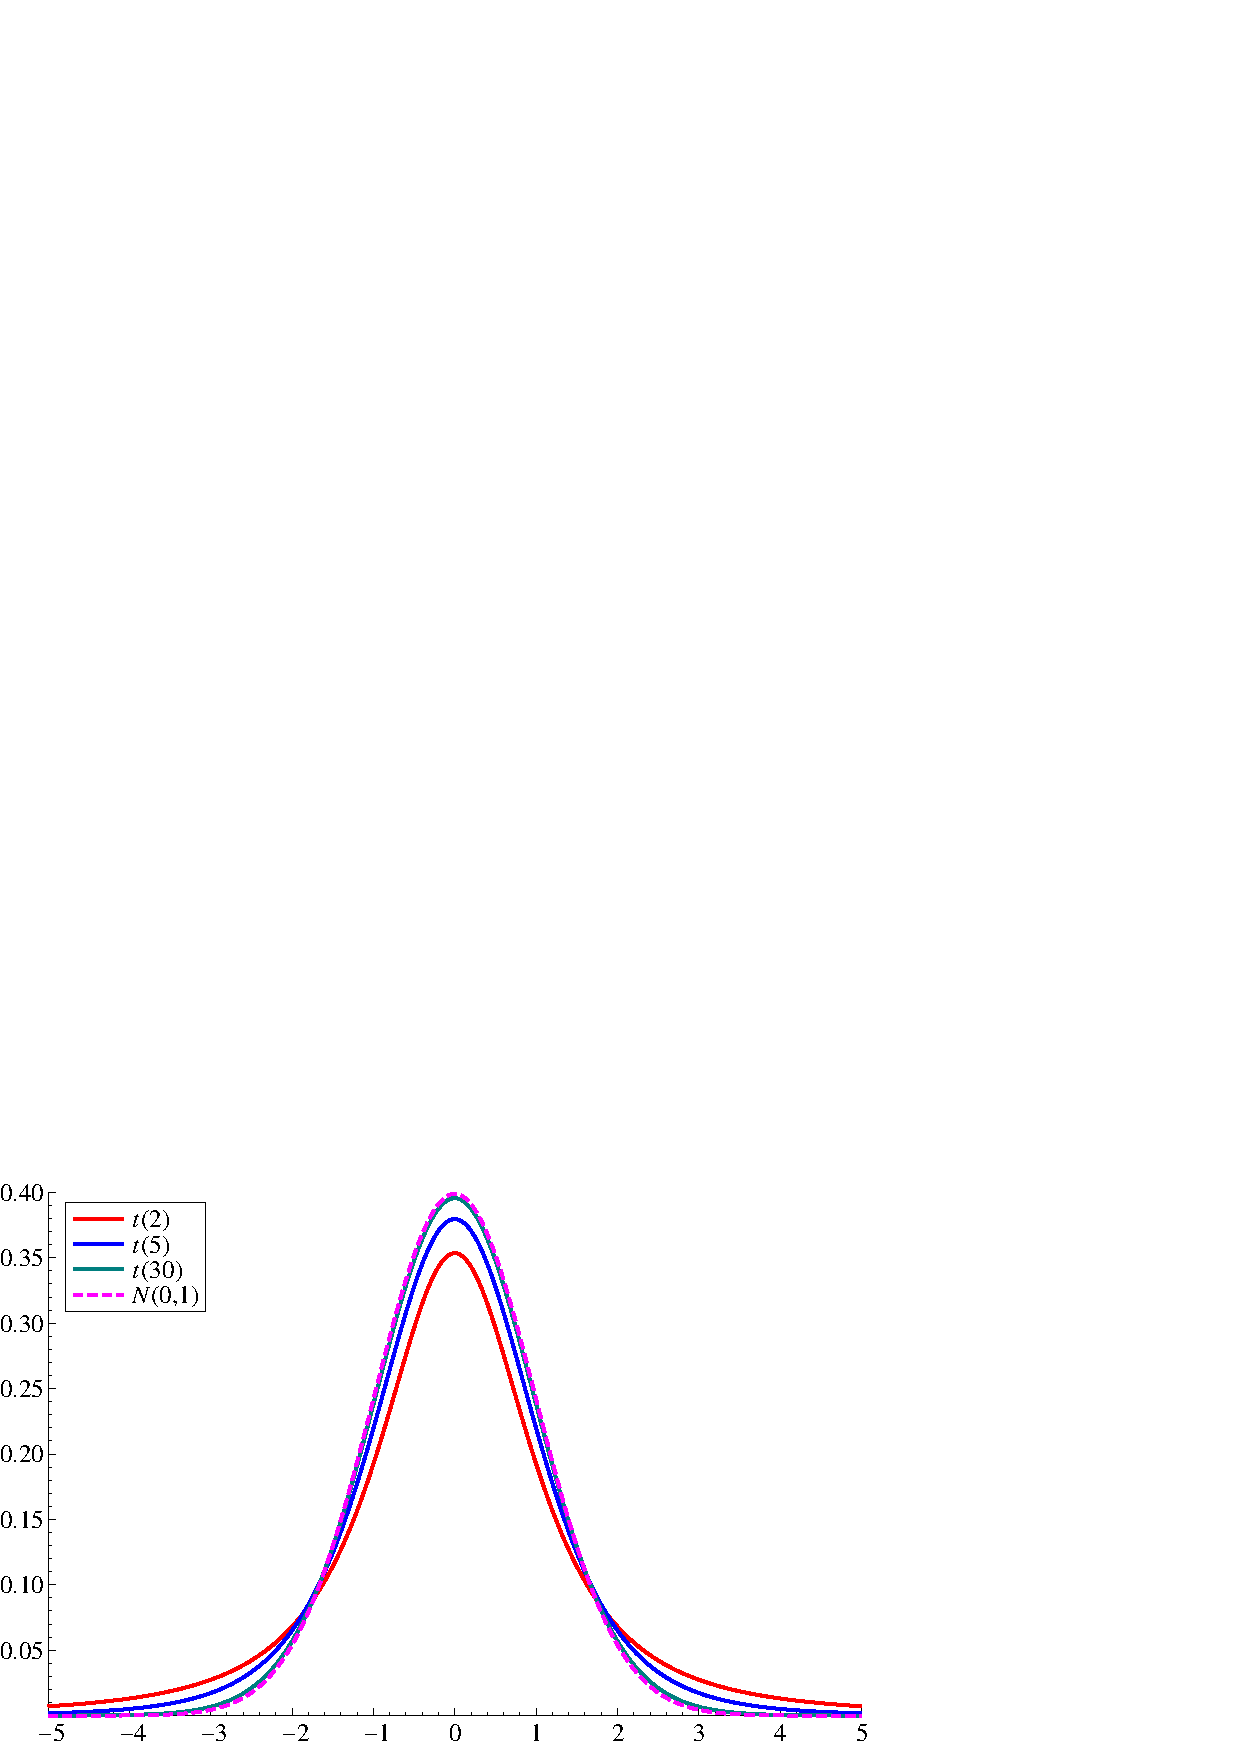
\includegraphics[height=2.5in]{Student}}
\end{block}

%TCIMACRO{\TeXButton{EndFrame}{\end{frame}}}%
%BeginExpansion
\end{frame}%
%EndExpansion

%TCIMACRO{\TeXButton{BeginFrame}{\begin{frame}}}%
%BeginExpansion
\begin{frame}%
%EndExpansion

\frametitle{VaR Methods: Standardized $t$ distribution}

\begin{itemize}
\item The GARCH model $R_{t+1}=\mu_{t+1}+\sigma _{t+1}z_{t+1}$, $\sigma
_{t+1}^{2}=\omega +\alpha R_{t}^{2}+\beta \sigma _{t}^{2}$, may be extended
to $z_{t}\sim \tilde{t}(d)$, where $d$ is an extra parameter that needs to be estimated.

%\item Alternatively, the GARCH model can be estimated as usual (assuming
%normality), and then the parameter $d$ can be estimated separately from the
%standardized residuals, either by quasi-ML or by matching the kurtosis to
%that of the data.

\item In practice this GARCH-$t$ model often gives a substantially better
fit than the Gaussian model. The main problem is that the standardized
residuals usually have an asymmetric distribution, with a longer left tail
than right tail.
\end{itemize}

%TCIMACRO{\TeXButton{EndFrame}{\end{frame}}}%
%BeginExpansion
\end{frame}%
%EndExpansion

\begin{frame}[fragile]
\begin{block}{Estimation of GARCH-$t$ in Python}
\tiny
\begin{verbatim}
                                                 Constant Mean - GARCH Model Results
                         ====================================================================================
                         Dep. Variable:                   log_return   R-squared:                       0.000
                         Mean Model:                   Constant Mean   Adj. R-squared:                  0.000
                         Vol Model:                            GARCH   Log-Likelihood:               -3036.13
                         Distribution:      Standardized Student's t   AIC:                           6082.26
                         Method:                  Maximum Likelihood   BIC:                           6111.41
                         No. Observations:                 2517
                         Date:                      Tue, Oct 10 2023   Df Residuals:                     2516
                         Time:                              16:27:43   Df Model:                            1
                         Mean Model
                         ====================================================================================
                         coef    std err          t      P>|t|    95.0% Conf. Int.
                         ------------------------------------------------------------------------------------
                         mu             0.0913  1.205e-02      7.578  3.501e-14 [6.768e-02,  0.115]
                         Volatility Model
                         ====================================================================================
                                          coef    std err          t      P>|t|      95.0% Conf. Int.
                         ----------------------------------------------------------------------------
                         omega          0.0286  6.564e-03      4.353  1.343e-05 [1.571e-02,4.144e-02]
                         alpha[1]       0.2171  2.891e-02      7.508  6.009e-14     [  0.160,  0.274]
                         beta[1]        0.7767  2.496e-02     31.114 1.551e-212     [  0.728,  0.826]
                         Distribution
                         ====================================================================================
                                          coef    std err          t      P>|t|  95.0% Conf. Int.
                         ------------------------------------------------------------------------------------
                         nu             5.4748      0.592      9.248  2.293e-20 [  4.314,  6.635]
                         ====================================================================================

                         Covariance estimator: robust
\end{verbatim}
\end{block}
\end{frame}

%TCIMACRO{\TeXButton{BeginFrame}{\begin{frame}}}%
%BeginExpansion
\begin{frame}%
%EndExpansion

\frametitle{VaR Methods: Standardized $t$ distribution}

\begin{itemize}
\item Let $\tilde{t}_{p}^{-1}(d)$ be $100p\%$ quantile of the
standardized $t$ distribution $\tilde{t}(d)$ and $t_{p}^{-1}(d)$ the
percentile $100p\%$ of the $t$ distribution $t(d).$

\item The implied VaR now is
\begin{equation*}
VaR_{t+1}^{p}=-\mu_{t+1} -\sigma _{t+1}\tilde{t}_{p}^{-1}(d)=-\mu_{t+1 }-\sigma _{t+1}\sqrt{\frac{%
d-2}{d}}t_{p}^{-1}(d),
\end{equation*}%
where, e.g., $\tilde{t}_{.01}^{-1}(6)=-2.566$.
\end{itemize}

%Alternative methods to allow for fatter tails in the standardized residuals
%are the Cornish-Fisher approximation, or extreme value theory. We will not
%consider those here.

%TCIMACRO{\TeXButton{EndFrame}{\end{frame}}}%
%BeginExpansion
\end{frame}%
%EndExpansion
%TCIMACRO{\TeXButton{BeginFrame}{\begin{frame}}}%
%BeginExpansion
\begin{frame}%
%EndExpansion

\begin{block}{Example: negative of the S\&P500 returns, with $1\%$ VaR
based on historical simulation, a rolling normal distribution, and a GARCH(1, 1) with both normal and $t$ errors}
\centerline{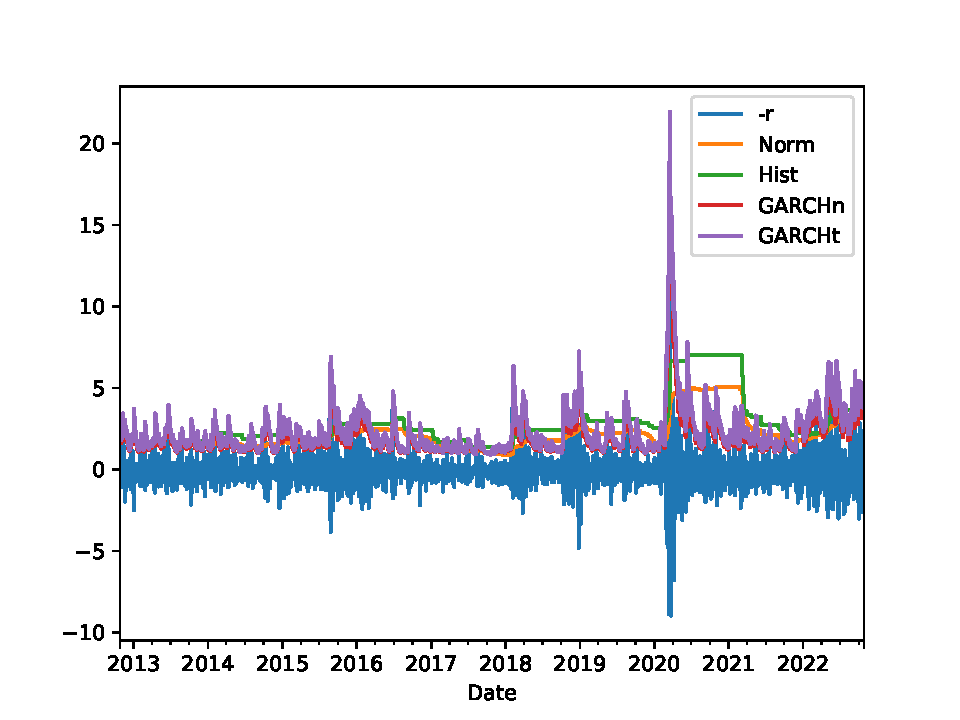
\includegraphics[height=2.2in]{VaRs}}
\end{block}
%TCIMACRO{\TeXButton{EndFrame}{\end{frame}}}%
%BeginExpansion
\end{frame}%
%EndExpansion
%%TCIMACRO{\TeXButton{BeginFrame}{\begin{frame}}}%
%%BeginExpansion
%\begin{frame}%
%%EndExpansion
%
%\begin{block}{QQ plot of standardized residuals against $\tilde{t}(d)$:}
%\centerline{\includegraphics[height=2.5in]{QQt.jpg}}
%\end{block}
%
%%TCIMACRO{\TeXButton{EndFrame}{\end{frame}}}%
%%BeginExpansion
%\end{frame}%
%%EndExpansion
\section{Expected Shortfall}\subsection*{}

%TCIMACRO{\TeXButton{BeginFrame}{\begin{frame}}}%
%BeginExpansion
\begin{frame}%
%EndExpansion

\frametitle{Expected Shortfall}

Limitations of Value at Risk:

\begin{itemize}
\item VaR is not informative about the magnitude of the losses if they
exceed the VaR. Two distributions could have the same $1\%$ VaR, but with
different left tails.

\item VaR is not \emph{\color{red}subadditive}: it is not guaranteed that
\begin{equation*}
VaR_{t+1}^{p}(X+Y)\leq VaR_{t+1}^{p}(X)+VaR_{t+1}^{p}(Y).
\end{equation*}
This means that VaR is not a \textquotedblleft coherent\textquotedblright\
risk measure.
\end{itemize}

%TCIMACRO{\TeXButton{EndFrame}{\end{frame}}}%
%BeginExpansion
\end{frame}%
%EndExpansion

%TCIMACRO{\TeXButton{BeginFrame}{\begin{frame}}}%
%BeginExpansion
\begin{frame}%
%EndExpansion

\frametitle{Expected Shortfall}

\begin{itemize}
\item With the rollout of Basel 3 which started on January 1st, 2023, the 1\% VaR is being replaced with the 2.5\%  \emph{%
\color{red}expected shortfall} (ES, a.k.a.\ CVaR), which addresses these problems.
\item It is defined as
\begin{equation*}
ES_{t+1}^{p}=-\mathbb{E}\left[ R_{t+1}|R_{t+1}<-VaR_{t+1}^{p}\right],
\end{equation*}
i.e., it represents the average of the losses exceeding the VaR.
\item Backtesting the ES is less straightforward than the VaR, and won't be discussed here.
\item Note however that a correctly specified ES requires that the VaR be correctly estimated in a first step,
so the methods discussed here remain relevant.
%\item When based on a (GARCH) model with conditional mean $\mu _{t+1}$,
%variance $\sigma _{t+1}^{2}$, and standardized returns $z_{t+1}$ with
%distribution $F(z)$, it becomes%
%\begin{equation*}
%ES_{t+1}^{p}=-\mu _{t+1}-\sigma _{t+1}E\left[ z_{t+1}|z_{t+1}<F_{p}^{-1}%
%\right] .
%\end{equation*}
%
%\item The main advantage of ES is that the shape of the tails of the
%distribution is taken into account. For example:
%
%\begin{itemize}
%\item $z_{t+1}\sim N(0,1)$: $\Phi _{.01}^{-1}=-2.33$ and $%
%E(z_{t+1}|z_{t+1}<\Phi _{.01}^{-1})=-2.67$;
%
%\item $z_{t+1}\sim $ $\tilde{t}(3)$: $\tilde{t}_{.01}^{-1}(3)=-2.62$ and $%
%E(z_{t+1}|z_{t+1}<\tilde{t}_{.01}^{-1}(3))=-4.04$.
%\end{itemize}
\end{itemize}

%TCIMACRO{\TeXButton{EndFrame}{\end{frame}}}%
%BeginExpansion
\end{frame}%
%EndExpansion
\section{Multi-Period VaR}\subsection*{}

%TCIMACRO{\TeXButton{BeginFrame}{\begin{frame}}}%
%BeginExpansion
\begin{frame}%
%EndExpansion

\frametitle{Multi-Period VaR}

\begin{itemize}
\item As we have seen, the one-day
VaR (and ES) can be determined analytically for the GARCH-$N(0,1)$ and GARCH-$\tilde{t}(d)$ models, when estimation is also based on
daily data.

\item However, in practice one often needs risk measures for multi-period
returns:%
\begin{equation*}
R_{t+1:t+K}=\sum_{k=1}^{K}R_{t+k}.
\end{equation*}%
For example, a horizon of two weeks ($K=10$ trading days) is common.
\end{itemize}
\end{frame}
\begin{frame}
\frametitle{Multi-Period VaR}
\begin{itemize}
\item Problem: even if the distribution of the one-period return is known (e.g., normal), that of $R_{t+1:t+K}$ is not (because the variance is not deterministic).
\item \emph{\color{red}Monte Carlo simulation} is a possible solution:
we let the computer generate a large number of scenarios of $K$ daily
returns, and compute from this the conditional distribution of the $K$-day
return, and hence the $K$-day VaR and ES.
\item Quick-and dirty practitioner solution: scale the one-day VaR with $\sqrt{K}$ (\er{square root of time rule}). This is strictly speaking only correct under normality.
\end{itemize}

%TCIMACRO{\TeXButton{EndFrame}{\end{frame}}}%
%BeginExpansion
\end{frame}%
%EndExpansion

%TCIMACRO{\TeXButton{BeginFrame}{\begin{frame}}}%
%BeginExpansion
%\begin{frame}%
%%EndExpansion
%
%\frametitle{Monte Carlo simulation and filtered historical simulation}
%
%Steps in Monte Carlo simulation:
%
%\begin{itemize}
%\item Estimate a normal GARCH(1,1) model based on returns $\{R_{1},\ldots
%,R_{t}\}$, yielding an estimate of $\sigma _{t}^{2}$.\
%
%\item Generate $N$ scenarios as follows: For $i=1,\ldots ,N$, draw
%independent $N(0,1)$ random variables $\{\check{z}_{i,1},\ldots ,\check{z}%
%_{i,K}\}$, and iterate between:%
%\begin{equation*}
%\left.
%\begin{array}{l}
%\check{\sigma}_{i,t+j}^{2}=\omega +\alpha \check{R}_{i,t+j-1}^{2}+\beta
%\check{\sigma}_{i,t+j-1}^{2}, \\
%\check{R}_{i,t+j}=\check{\sigma}_{i,t+j}\check{z}_{i,j},%
%\end{array}%
%\right\} \qquad j=1,\ldots ,K.
%\end{equation*}
%
%\item This leads to $N$ simulated multi-period returns:%
%\begin{equation*}
%\check{R}_{t+1:t+K}^{i}=\sum_{j=1}^{K}\check{R}_{i,t+j}, \qquad i=1,\ldots,N.
%\end{equation*}
%
%\item Minus the $100p$th percentile of these $N$ simulations is an estimator
%of $VaR_{t+1:t+K}^{p}$.
%\end{itemize}
%
%%TCIMACRO{\TeXButton{EndFrame}{\end{frame}}}%
%%BeginExpansion
%\end{frame}%
%%EndExpansion
%
%%TCIMACRO{\TeXButton{BeginFrame}{\begin{frame}}}%
%%BeginExpansion
%\begin{frame}%
%%EndExpansion
%
%\frametitle{Monte Carlo simulation and filtered historical simulation}
%
%\begin{itemize}
%\item The same approach can be followed with another distribution for $%
%\check{z}_{i,j}$, such as the Student's $\tilde{t}(d)$ distribution.
%
%\item To avoid misspecification of the distribution of $z_{t}$, one can use
%\emph{\color{red}filtered historical simulation}, which means drawing $\hat{z%
%}_{i,j}$ from the empirical distribution of the standardized residuals $\{%
%\hat{z}_{t+1-j},j=1,\ldots ,m\}$ ($m\leq t$).
%
%\item This is a combination of a parametric GARCH model and the
%non-para\-metric historical simulation technique. This allows, e.g., for
%different left and right tails of the distribution. As usual, the last $m$
%observations need to be \textquotedblleft representative\textquotedblright .
%\end{itemize}
%
%%TCIMACRO{\TeXButton{EndFrame}{\end{frame}}}%
%%BeginExpansion
%\end{frame}%
%%EndExpansion
\section[Backtesting]{Backtesting Value at Risk}\subsection*{}

%TCIMACRO{\TeXButton{BeginFrame}{\begin{frame}}}%
%BeginExpansion
\begin{frame}%
%EndExpansion

\frametitle{Backtesting Value at Risk}

\begin{itemize}
\item The Basel Committee requires that methods to evaluate VaR be
backtested.

\item They recommend constructing the 1\% VaR over the last 250 trading days
($\approx $ 1 year), and counting the number of times that losses have exceeded the
day's VaR figure (termed \er{exceptions} or \er{violations} ).

\item A method is said to lie in the:

\begin{itemize}
\item \emph{\color{green}Green zone}, in case of 0--4 exceptions;

\item \emph{\color{orange}Yellow zone}, in case of 5--9 exceptions;

\item \emph{\color{red}Red zone}, in case of 10 exceptions or more.
\end{itemize}
\item The capital charge for the bank changes according to the zone.
\end{itemize}

%TCIMACRO{\TeXButton{EndFrame}{\end{frame}}}%
%BeginExpansion
\end{frame}%
%EndExpansion

%TCIMACRO{\TeXButton{BeginFrame}{\begin{frame}}}%
%BeginExpansion
\begin{frame}%
%EndExpansion

\frametitle{Backtesting Value at Risk}

How can we test if a VaR method is accurate?

\begin{itemize}
\item Define the \emph{\color{red}hit sequence}%
\begin{equation*}
I_{t+1}=\left\{
\begin{array}{cc}
1, & \text{if }R_{t+1}<-VaR_{t+1}^{p}, \\
0, & \text{if }R_{t+1}>-VaR_{t+1}^{p}.%
\end{array}%
\right.
\end{equation*}

\item Consider a test period that covers $t+1\in \{1,\ldots ,T\}$, then the
number of exceptions is given by $T_{1}=\sum_{t=1}^{T}I_{t}.$

\item The proportion of exceptions is given by $\hat{\pi}=T_{1}/T$ which is
an estimator of $\mathbb{P} \left ( R_{t+1}<-VaR_{t+1}^{p}\right )$.

\item Recall that if the model that generated $VaR_{t+1}^{p}$ is correctly
specified, then
\begin{equation*}
\mathbb{P} \left ( R_{t+1}<-VaR_{t+1}^{p}\right ) =p,
\end{equation*}
independent of any information at time $t$.
\end{itemize}

%TCIMACRO{\TeXButton{EndFrame}{\end{frame}}}%
%BeginExpansion
\end{frame}%
%EndExpansion

%TCIMACRO{\TeXButton{BeginFrame}{\begin{frame}}}%
%BeginExpansion
\begin{frame}%
%EndExpansion

\frametitle{Backtesting Value at Risk}

\begin{itemize}
\item Hence, under the null hypothesis of correct specification, the hits
$\{I_{t+1}\}$ are independent Bernoulli random variables, and so $%
T_{1}=\sum_{t=1}^{T}I_{t}$ has a Binomial($T$, $p$) distribution.

\item We can test this hypothesis (e.g., with $p=0.01$) based on the $t$%
-statistics
\begin{equation*}
t_{0}=\frac{\hat{\pi}-p}{\sqrt{p(1-p)/T}}\qquad \text{or\qquad }t=\frac{\hat{%
\pi}-p}{\sqrt{\hat{\pi}(1-\hat{\pi})/T}}.
\end{equation*}

\item Under $H_{0}$ their asymptotic distribution is $N(0,1).$

\item The second $t$-statistic is equal (up to degrees-of-freedom
correction) to the OLS-based $t$-statistic in regression of $I_{t+1}-p$ on a
constant; see exercises.
\end{itemize}

%TCIMACRO{\TeXButton{EndFrame}{\end{frame}}}%
%BeginExpansion
\end{frame}%
%EndExpansion

%TCIMACRO{\TeXButton{BeginFrame}{\begin{frame}}}%
%BeginExpansion
\begin{frame}%
%EndExpansion

\frametitle{Backtesting Value at Risk}

\begin{itemize}
\item The previous test only checks \emph{\color{red}unconditional}
coverage, i.e., $\mathbb{P} ( I_{t+1} = 1 ) =p$ \emph{\color{red}on average}.
However, misspecification often is due to the fact that the hits $I_{t+1}$
are not independent over time.

\item If exceptions are clustered, then if today there was an exception a
risk manager can infer that the probability of occurring another exception
tomorrow is higher than $p$. Hence, there is misspecification.

\item We would like to test if the VaR violations are \emph{\color{red}%
independent} over time, the null hypothesis is
\begin{equation*}
H_{0}:\mathbb{P} (I_{t+1}=1|I_{t}=1)=\mathbb{P} (I_{t+1}=1|I_{t}=0),
\end{equation*}
which implies $\mathbb{P} (I_{t+1}=0|I_{t}=0)=\mathbb{P} (I_{t+1}=0|I_{t}=1) $.
\end{itemize}

%TCIMACRO{\TeXButton{EndFrame}{\end{frame}}}%
%BeginExpansion
\end{frame}%
%EndExpansion

%TCIMACRO{\TeXButton{BeginFrame}{\begin{frame}}}%
%BeginExpansion
\begin{frame}%
%EndExpansion

\frametitle{Backtesting Value at Risk}

\begin{itemize}
\item Also of interest is to test if the VaR violations are independent over
time and if the number of violations is correct (\emph{\color{red}%
conditional coverage})
\begin{equation*}
H_{0}:\mathbb{P} (I_{t+1}=1|I_{t}=1)=\mathbb{P} (I_{t+1}=1|I_{t}=0)=p.
\end{equation*}

\item A simple approach to test these hypotheses is to consider the linear
regression model
\begin{equation*}
I_{t+1}-p=b_{0}+b_{1}I_{t}+e_{t+1}
\end{equation*}

\item The \emph{\color{red}conditional coverage} hypothesis is equivalent to
$H_{0}:b_{0}=b_{1}=0$ and can be tested using a $F$-test.

\item The \emph{\color{red}independence} hypothesis is equivalent to $%
H_{0}:b_{1}=0$ and can be tested using a $t$-test.
\end{itemize}

%TCIMACRO{\TeXButton{EndFrame}{\end{frame}}}%
%BeginExpansion
\end{frame}%
%EndExpansion

%TCIMACRO{\TeXButton{BeginFrame}{\begin{frame}}}%
%BeginExpansion
\begin{frame}%
%EndExpansion

\frametitle{Backtesting Value at Risk}



\begin{block}{Results for S\&P500 returns, 4 different methods}
\begin{center}
	\begin{tabular}{l|rrrr}
		\toprule
		{} &       Norm &       Hist &     GARCHn &    GARCHt \\
		\midrule
		$100\cdot \hat{\pi}$ &  3.10 &   1.67 &   2.54 &  1.71 \\
		$t(\pi =0.01)$    &   6.08 &   2.62 &   4.92 &  2.74 \\
		$\hat{b}_{1}$   &   0.07 &   0.10 &   0.00 &  0.03 \\
		$t(b_{1}=0)$ &   3.71 &   5.25 &   0.30 &  1.50 \\
		$F(b_{0}=b_{1}=0)$    &  25.45 &  17.24 &  12.13 &  4.89 \\
		\bottomrule
	\end{tabular}
\end{center}
\small The critical values for the $t$ and $F$ tests are, respectively, $\pm 1.96$ and $3.00$.\\
The GARCHt model fares best, even though correct conditional coverage is still rejected. This is likely driven by the incorrect unconditional coverage, since independence is not rejected. This means that we'd need a different distribution, such as a Skew-$t$.
\end{block}
%TCIMACRO{\TeXButton{EndFrame}{\end{frame}}}%
%BeginExpansion
\end{frame}%
%EndExpansion

\section{Epilogue}
\begin{frame}
\frametitle{Learning Goals}
Students
\begin{itemize}
\item know the definitions of VaR and Expected Shortfall,
\item understand the limitations of the VaR,
\item are able to construct VaR forecasts based on various methods,
\item and are able to backtest VaR forecasts.
\end{itemize}
\end{frame}
\frameit{Homework}{
\item Exercise 6
\item \er{Assignment 1}. Deadline: Sunday after next, 11.59 p.m.
}
\end{document}
